%%% Local Variables:
%%% mode: latex
%%% TeX-master: t
%%% End:

% !Mode:: "TeX:UTF-8"

\chapter{考虑温度对漏电流功耗影响的MPSoC结构级热分析方法}
\label{cha:SSTA}


\section{多核芯片热分析研究基础}
\label{sec:SSTAbasic}

\subsection{多核架构及其电热分布}

目前多核CPU采用同质架构,即每个核拥有相同的逻辑功能模块、容量相同的专享缓存(cache),占有相同的内核面积, 同时共享最后一级缓存(last level cache,LLC)缓存、I/O等功能模块。 每个核具有相同数量的工作模式,但不同的工作模式具有不同的能耗,即每个核具有一个全速高能模式外, 还具有多个节能程度不同的节能模式。
在每个核内,一般都具有一个功耗密度最大的逻辑功能模块、一个指令L1缓存和一个数据L1缓存,其功耗密度次之, 一个功耗密度最小的L2缓存。由于注入的热量大,每个核的热点(温度最高点)出现在逻辑功能模块,所以在物理设计中, 逻辑功能模块一般要布放在散热条件好的芯片边沿处,而将功耗密度最小的LLC布放在散热条件最差的芯片中央, 以降低芯片的热点温度。 图~\ref{fig:ev6}为Alpha 21264芯片的物理布局~\onlinecite{TemMicroArch},

\begin{figure}[H]
  \centering
  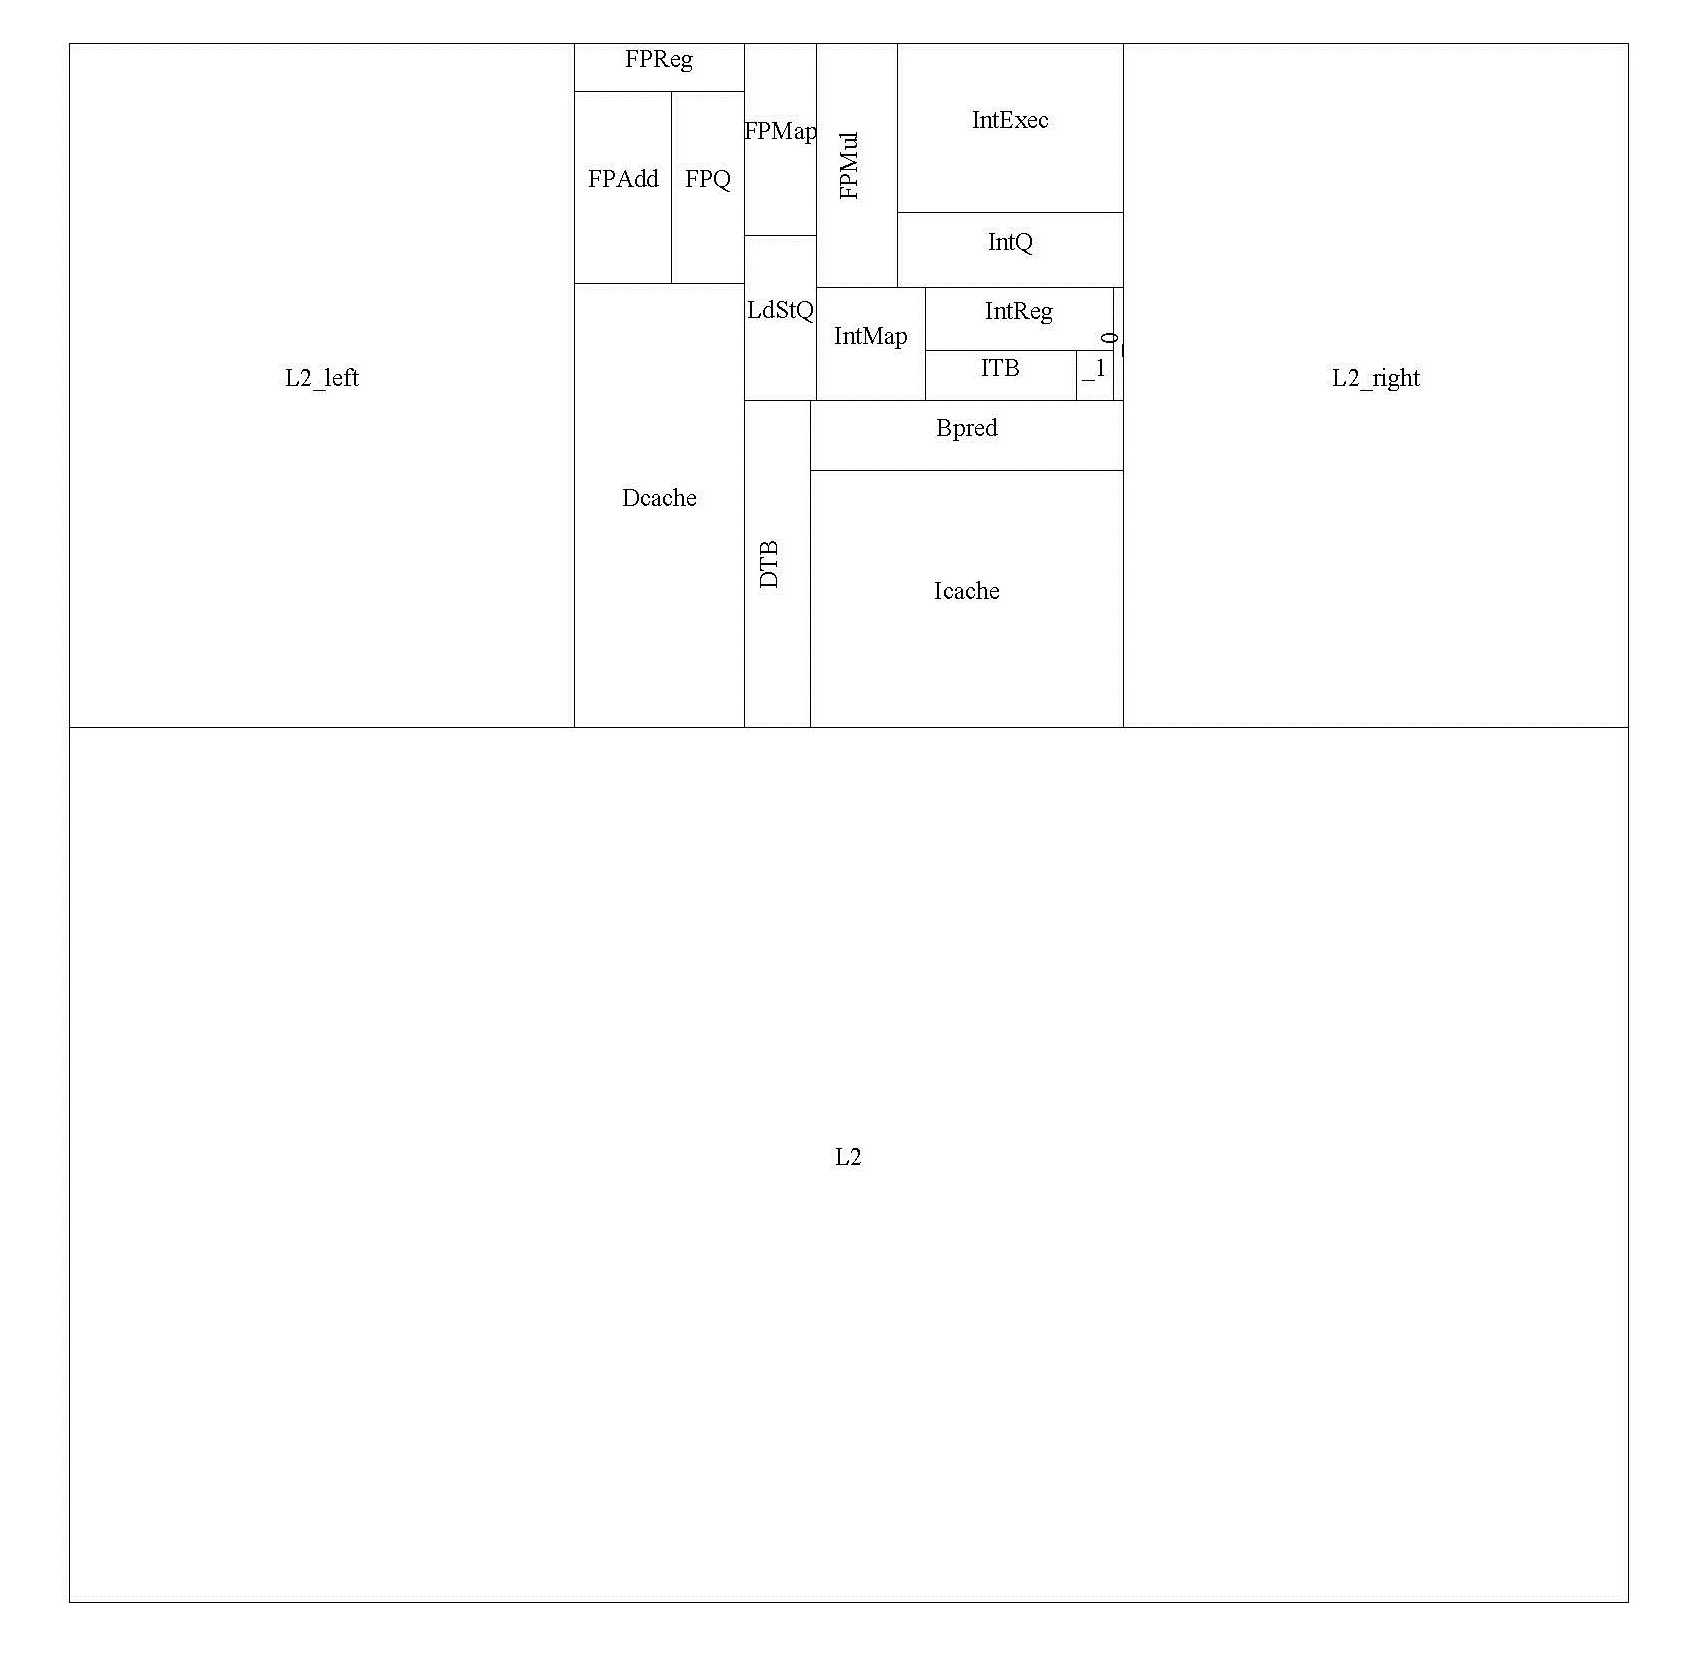
\includegraphics[width=1\textwidth,height=0.7\textheight]{EV6}
  \caption{Alpha21264芯片的物理布局}
  \label{fig:ev6}
\end{figure}


\subsection{芯片热分析及HotSpot模块级模型}

在MPSoC结构级热分析中,一般采用稳态热分析方法计算温度分布,以降低计算复杂度[7,8]。 对于稳态热分析而言,将芯片的功耗分布作为注入的热流向量$\mathbf{P}$,对芯片进行离散化建模后, 可以获得节点之间的热导矩阵$\mathbf{G}$, 目前多采用如下的稳态热分析方程计算节点温度分布向量$\mathbf{T}$:
\begin{equation}
\label{equ:chap4:gtp}
\mathbf{G} \times \mathbf{T} = \mathbf{P}
\end{equation}
对于多核实时功耗温度管理(dynamic power and temperature management, DPTM)研究\onlinecite{ThmBefMulCrFlrPlLimSty,TemSupVolPerfPowMdlMicroLvl}, 目前广泛采用Skadron等的HotSpot热分析模型\onlinecite{TemMicroArch}进行构建热导矩阵$\mathbf{G}$, 并采用式~\ref{equ:chap4:gtp}进行计算。 HotSpot采用基于等效热导的电路模型,将体系结构级的功能块作为分析热点的对象。 一种直观的对应芯片以及热封装的物理结构的具体建模例子如图~\ref{fig:hotspot-model} 所示\onlinecite{ThrOptTskAllocThemConstMulPro}。电路模型在垂直热传导方向上有3层:内核(die)层、扩热(heat spreader)层、与散热片(heatsink)层,另外加入第4层热对流(heat convector)层,即与环境温度的接口。内核层根据芯片的几何布局被分为块;扩热层分为5块: 与内核层完好对应的Rsp以及4块呈梯形状的环绕块;散热片层按照与扩热层相似的划分方法,分为Rhs以及4个环绕块; 最后,从热封装到外界环境的热对流层由Rconvection表示。层与层之间模型刻画由内核直至封装及外界环境的热流; 层内水平模型刻画相邻模块间的热扩散。内核层产生的功耗等效为每个模块中心的电流源。 建模完成后,通过电路分析可得到芯片的温度分布。 用HotSpot计算分析Alpha 21264芯片的温度分布如图~\ref{fig:ev6-grid-temp-surf}所示。

\begin{figure}[H]
  \centering
  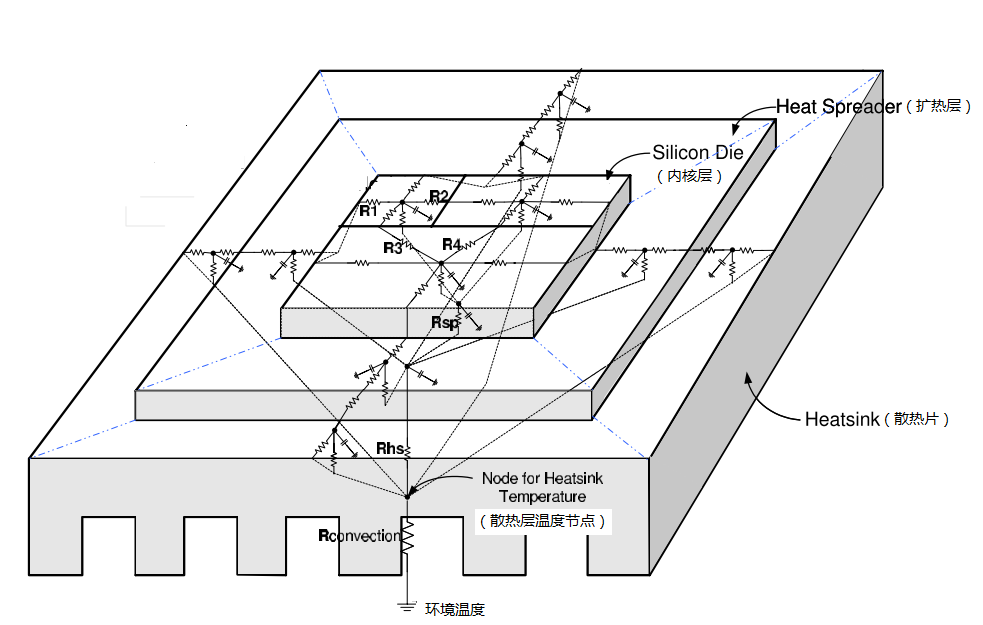
\includegraphics[width=1\textwidth,height=0.45\textheight]{HOTSPOT-MODEL}
  \caption{IC热分析的HotSpot分析模型}
  \label{fig:hotspot-model}
\end{figure}

\begin{figure}[H]
  \centering
  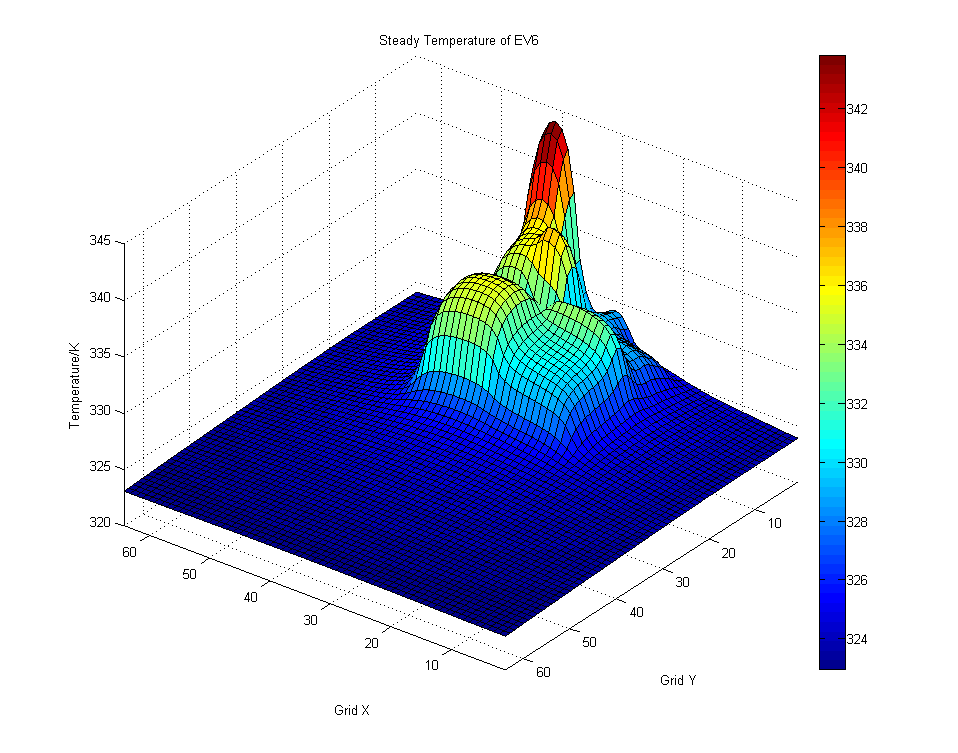
\includegraphics[width=1\textwidth,height=0.6\textheight]{EV6-GRID-TEM-SURF}
  \caption{Alpha21264芯片的温度分布}
  \label{fig:ev6-grid-temp-surf}
\end{figure}


\subsection{电热耦合效应:温度对漏电流功耗的影响}
正如~\ref{sec:power}节中,式~\ref{equ:chap2:active_power_simplified}、~\ref{equ:chap2:leakage_power} 所定性与定量地描述那样,芯片功耗由动态功耗$P_{dynamic}$与静态功耗$P_{leakage}$两部分组成, 随着工艺的提高,$P_{leakage}$已成为芯片功耗的主要贡献者。 而工作温度$T$的升高可以明显增大$P_{leakage}$,此现象称之为电热耦合效应。考虑电热耦合效应的热分析过程中, 需要对$T-P$采用迭代计算。
如~\ref{fig:tp-iteration}所示,对于一个16核CPU的测例(其具体的实验参数设置见本文后面的3.1部分),采用迭代算法来逼近最终的精确解, 与不考虑电热耦合效应的初始解相比,芯片最高温度与静态功耗都有了明显的增加, 这表明在芯片的温度分析中、必须考虑温度对静态功耗的影响,否则,将会产生较大的分析误差。 同时,与不考虑电热耦合效应的温度分析算法相比, 由于考虑电热耦合效应的温度分析算法需要采用7次迭代计算才能获得精确解, 所以其算法复杂度是对比算法的7倍;因此降低考虑电热耦合效应的温度分析算法复杂度就具有非常重要的研究意义
\begin{figure}[H]
  \centering
  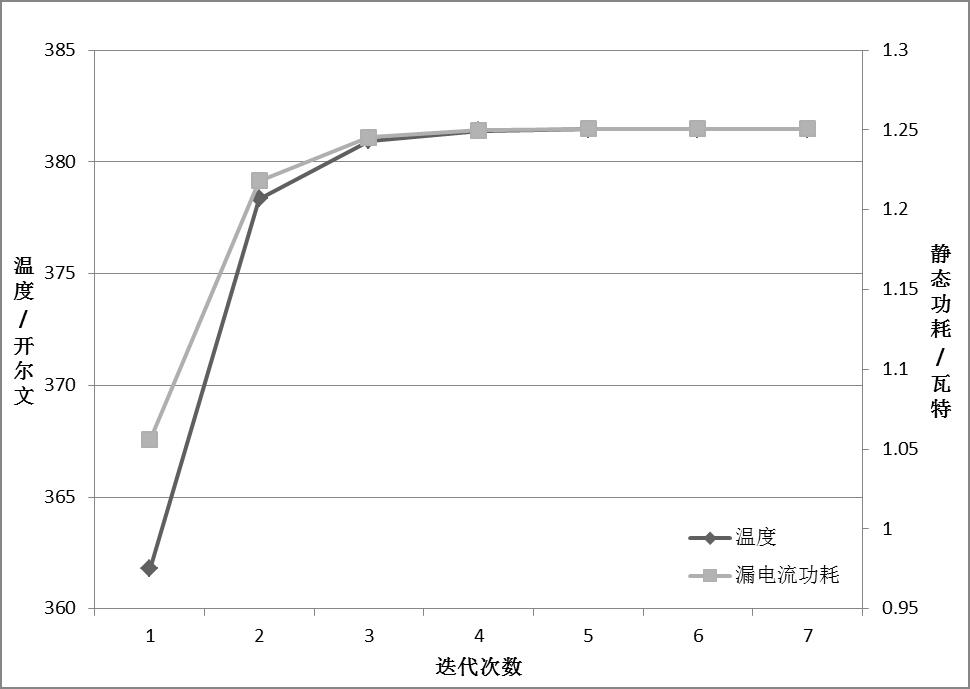
\includegraphics[width=1\textwidth,height=0.6\textheight]{TP-ITERATION}
  \caption{考虑电热耦合效应的多核芯片最高温度与静态功耗的迭代求解}
  \label{fig:tp-iteration}
\end{figure}


\section{3种MPSoC结构级热分析方法}
\label{sec:SSTAmethod}

\subsection{模块级热分析方法BloTAM}
为了对功能模块进行热分析建模,按照~\ref{fig:hotspot-model}对HotSpot的多核芯片热分析模型, 采用等效电路的方法对其进行进一步简化, 为此本文假设:每个功能模块内的功耗与温度分布是均匀的,以该模块中心点的温度作为该模块的温度, 并将功耗密度乘以面积作为该模块的功耗,加于模块中心点。
在本文工作中,将模块$i$的功耗$P_{i,i}$作为注入热源。对于多核芯片,如果仅在模块$i$加上幅值为$P_{i,i}$的阶跃激励, 其他模块均不加激励,则可以使用HotSpot模拟器获得所有模块的温度$T_{j,i}$响应曲线。 先根据$T_{i,i}$的最终收敛值$\overline{T}_{i,i}$ 可以计算出模块$i$的等效热阻$R_{i,i}$,计算公式为~\ref{equ:chap4:blotam-rii}
\begin{equation}
\label{equ:chap4:blotam-rii}
R_{i,i} = \frac{\overline{T}_{i,i}}{P_{i,i}}
\end{equation}
再根据等效热阻$R_{i,i}$以及模块$j$功耗$P_{j,j}$的阶跃激励作为单一注入热源所得到的$\overline{T}_{i,j}$, 可以采用~\ref{equ:chap4:blotam-rij}公式计算出反映$P_{j,j}$对模块$i$温度作用关系的等效热阻$R_{i,j}$,
\begin{equation}
\label{equ:chap4:blotam-rij}
R_{i,j} = \frac{\overline{T}_{i,j}}{P_{j,j}}
\end{equation}
最后根据所获得的参数$R_{i,i}$与$R_{i,j}$ ,可以计算$P_{j,j}$对模块$i$温度计算产生影响的等效热源$P_{i,j}$:
\begin{equation}
\label{equ:chap4:blotam-pij}
P_{i,j} = \frac{\overline{T}_{i,j}}{\overline{T}_{i,i}}P_{i,i} = \frac{R_{i,j}\times P_{j,j}}{R_{i,i}\times P_{i,i}}P_{i,i}=\frac{R_{i,j}}{R_{i,i}}P_{j,j}
\end{equation}
因此,按照图~\ref{fig:multicore-temp-model}中所给出的单模块温度分析模型,可以列出如下热分析表达式:
\begin{equation}
\label{equ:chap4:blotam-tii}
T_{i,i} = R_{i,i}\sum\limits_{j=1}^N P_{i,j} = R_{i,i}\widehat{P_{i}}
\end{equation}
其中$N$为多核芯片中的功能模块数目,$\widehat{P_{i}} = \sum\limits_{j=1}^N P_{i,j}$为模块$i$的等效热源,由于一个模块只有一个等效热源, 可见式~\ref{equ:chap4:blotam-tii}提供的单模块热分析模型兼容了经典的单核(单模块)热分析模型[16]。 从式~\ref{equ:chap4:blotam-tii}可知:BloTAM方法的算法时间复杂度与空间复杂度均为$O(N^2)$,即算法复杂度为$O(N^2)$。
\begin{figure}[H]
  \centering
  
\includegraphics[width=1.0\textwidth,height=0.35\textheight]{MULTICORE-TEMP-MODEL}
  \caption{多核DPTM的单模块与单核热分析等效简化模型}
  \label{fig:multicore-temp-model}
\end{figure}

\subsection{核级热分析方法CorTAM}








\subsection{考虑核内模块相互影响的改良核级热分析方法BiCorTAM}



